\documentclass[
  11pt,
  letterpaper,
   addpoints,
   %answers
  ]{exam}

\usepackage{../exercise-preamble}
\usepackage{float}

\begin{document}

\noindent
\begin{minipage}{0.47\textwidth}

\includegraphics[width=\textwidth]{../fcfm_die}
\end{minipage}
\begin{minipage}{0.53\textwidth}
\begin{center} 
\large\textbf{Análisis de Sistemas Dinámicos y Estimación} (EL3103) \\
\large\textbf{Examen} \\
\normalsize Prof.~Heraldo Rozas.\\
\normalsize Prof.~Aux.~Erik Saez - Maximiliano Morales
\end{center}
\end{minipage}

\vspace{0.5cm}
\noindent
\vspace{.85cm}
%--------------------------------------------------------------------------
\begin{questions}
    %--------------------------
    \question Se considera un circuito RLC acoplado como el mostrado en la Figura 1. Este tipo de circuitos se encuentra comúnmente en sistemas electrónicos utilizados para filtrar señales, almacenar energía o controlar la resonancia en aplicaciones industriales y de telecomunicaciones. En este ejercicio, se desea analizar el modelo matemático del sistema, evaluar su controlabilidad y diseñar estrategias para lograr el comportamiento deseado mediante controladores y observadores de estado. Esto permite simular problemas reales como los ajustes necesarios en el diseño cuando hay restricciones físicas o fallas en los sensores.

    \begin{figure}[h!]
        \centering
        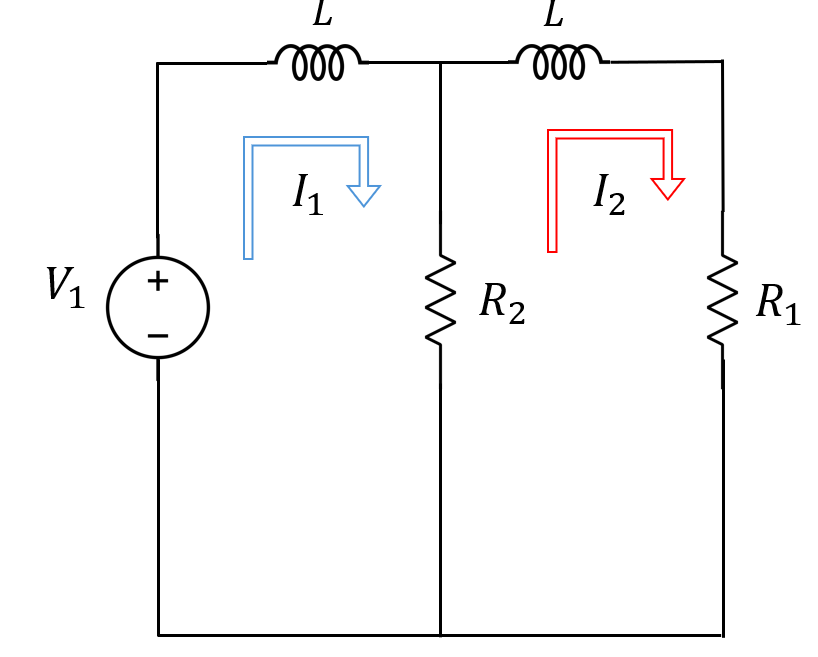
\includegraphics[width=0.4\textwidth]{Examen_1}
        \caption{Circuito RLC.}
    \end{figure}
    Dado el circuito mostrado en la Figura 1 y considerando que $R_{1}= 1$ $R_{2} = 0.5$ y $L=100[mA]$, se requiere resolver lo siguiente:

    \begin{enumerate}
        \item[\textbf{a)}] Demuestre  \( \mathbf{A}, \mathbf{B}, \mathbf{C} \) y \( \mathbf{D} \) del sistema en representación de espacio de estados vienen dadas por:
        \begin{align}
            \mathbf{A} =
            \begin{bmatrix}
            -5 & 5 \\
            5 & -15
            \end{bmatrix}, \quad
            \mathbf{B} =
            \begin{bmatrix}
            1 \\
            0
            \end{bmatrix}, \quad
            \mathbf{C} =
            \begin{bmatrix}
            0 & 1
            \end{bmatrix}
        \end{align}
        
        \item[\textbf{b)}] Analice si el sistema es controlable, observable y si cumple la condición de estabilidad BIBS.
    
        \item[\textbf{c)}] Debido a especificaciones en el diseño, es necesario que los polos de la matriz \( \mathbf{A} \) del sistema se ubiquen en  \( \lambda_{1,2} = -15 \pm 15j \). Diseñe un controlador que garantice que los polos cumplan esta condición.
    
        \item[\textbf{d)}] Debido a un problema de fabricación, no es posible medir directamente los estados del sistema. Sin embargo, sí se puede acceder a la salida. Diseñe un observador de estados que estime los valores de las variables de estado determinadas en a) basándose únicamente en las salidas del sistema.
    
        \item[\textbf{e)}] Dibuje un diagrama que integre tanto el controlador como el observador en el sistema. Asegúrese de mostrar claramente la interacción entre las señales de entrada, los estados estimados y las salidas.
    \end{enumerate}
    %--------------------------
    \begin{solution}
        \subsection*{Resolucion 1.1}
    \end{solution}

    %--------------------------
    \begin{solution}
        \subsection*{Resolucion 2.1}
    \end{solution}
    %--------------------------

    %--------------------------
\end{questions}

\end{document}